\section{Geolog\'ia}
En la cuenca hidrogr\'afica de la quebrada La Linda se encuentran 3 unidades geol\'ogicas, una sedimentaria la cual corresponde al Miembro Urrao de la Fm. Penderisco y aguas arriba de la Quebrada La Linda se encuentra el Batolito Farallones.\\

\textbf{Batolito Farallones.Tmcf}
Ubicado al Sur del Stock de Cerro plateado de y de formaci\'on contemporanea a este. El Batolito Farallones recibe su nombre por encontrarse lozalizado al Este de la localidad de Farallones.
El Batolito Farallones de edad Mioceno datado por el m\'etodo $K/Ar$ como originado hace 11 +- 2 m.a. \cite{farallones}. Presenta una aureola de contacto extensa (500m aprox), fuertemente fallada y plegada con los sedimentos cret\'acicos que lo rodean en su extremo norte. Su altura alcanza apr\'oximadamente los 3400msnm exhibiendo escarpes casi totalmente verticales.
Su clasificaci\'on se determin\'o como intrusivo monzonitico.
 

\textbf{Fm. Penderisco Miembro Urrao. Ksaau}
La sedimentaci\'on de la formaci\'on penderisco se ubica entre el cretaceo temprano a tardio como producto de flujos de turbiedad.
Est\'a compuesta por estratos de rocas que var\'ian en calibre desde areniscas pasando por limolitas y lodolitas (siendo esta la facie predominante) hasta chert, este \'ultimo se presenta frecuentemente como interestratificaciones finas. Se presentan igualmente conglomerados de tama\~no de clasto altamente variable (polim\'ictico), los cuales presentan espesores y arreglos altamente variables.
Tanto algunas lodolitas como estratos de areniscas exhiben estructuras de polaridad como estratificaci\'on cruzada, siendo la 
Su estructura fue fuertemente modificada por el emplazamiento del Batolito Farallones en en Ne\'ogeno temprano. \cite{urrao}En la figura \ref{fig:mapageo}

\textbf{Fm. Barroso. Kvb}

Las rocas de esta formaci\'on abarcan una extensa variedad composicional. Desde basaltos y rocas andes\'iticas contenidas en flujos l\'avicos hasta rocas afan\'iticas. Mineralogicamente se presentan con mayor ocurrencia espilitas seguidas de diabasas, basaltos porfidicos, aglomerados y brechas.

Hacia el este de la Plancha 135 se presentan rocas masivas y frescas de coloraci\'on oscura con alto grado de deformaci\'on. Su composicion mineral\'ogica contiene clinopiroxenos y ortopiroxenos, plagioclasa, ilmenita, clorita y leucoxeno.

En la zona de trabajo se presenta en un punto aislado sobre la v\'ia que de Ciudad Bolivar conduce a Quibd\'o.
All\'i su ocurrencia se presenta en forma de diabasa altamante fracturada y de color oscuro, con intercalaciones de chert. \cite{barroso}, 




La descripci\'on geol\'ogica retomada de la informaci\'on bibliogr\'afica oficial sirvi\'o en los ensayos preliminares del software Scoops3D (secci\'on \ref{chap:pruebas preliminares}) como referencia para seleccionar los par\'ametros de resistencia a usar en dichos ensayos.

\begin{figure}[H]
\centering
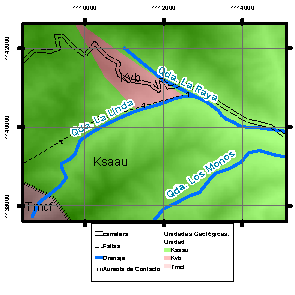
\includegraphics[scale=0.5]{img/geologia.pdf}
\caption{Mapa geol\'ogico de la zona de estudio basado en \cite{geol}. Se marca la ruta realizada durante la salida de campo y las estaciones de donde se tomaron las muestras para ensayos de laboratorio   }
\label{fig:mapageo}
\end{figure}


